\section{Energy resolution boost}
\label{Result}
The mean and standard deviation of parameters of 9 MCP-PMTs are summarized in Table~\ref{tab:summary}
\begin{table}
    \centering
    \caption{charge and time characteristic of MCP-PMTs}
    \label{tab:summary}
    \begin{tabular}{c| r @{$\pm$} l}
        Parameter&\multicolumn{2}{c}{Mean$\pm\sigma$}\\
        \hline
        $G_1$/1E7&1.17&0.07\\
        $G$/1E7&2.14&0.16\\
        $\mathrm{Res}_1$&0.25&0.02\\
        Res&0.69&0.03\\
        TTS/ns&1.82&0.09\\
        DCR/kHz&4.5&1.3\\
        $\tau_{\mathrm{ser}}$/ns&7.2&1.0\\
        $\sigma_{\mathrm{ser}}$/ns&1.62&0.06\\
        relative PDE&1.71&0.06\\
        $R_{\mathrm{pre}}$&0.00&0.00\\
        $R_{\mathrm{after}}$&0.02&0.01\\
        \hline
    \end{tabular}
\end{table}
\begin{table}
    \centering
    \caption{Parameters of after-pulse}
    \label{tab:afterpulse}
    \begin{tabular}{c|c|c|c|c}
        \hline
        &1st peak&2nd peak&3rd peak&4th peak\\
        $t_i$/ns&307$\pm$7&535$\pm$40&1194$\pm$34&1724$\pm$27\\
        $A_i/A_1$&0.53$\pm$0.22&0.96$\pm$0.44&1.9$\pm$&1.2\\
        $\sigma_i$/ns&11$\pm$4&66$\pm$40&50$\pm$30&69$\pm$28\\
        \hline
    \end{tabular}
\end{table}

Assume the number of expected photons $N$ on PMT obeys Poisson distribution $\pi~(\mu_N)$. Energy $E$ of Event proportional to $N=k\eta E$, in which $k$ is a factor that is relate to light yield and light transportation. The photon detection efficiency of PMT is $\eta$ and the single PE charge distribution is Gaussian distribution $G(\mu_C,\sigma_C^2)$. The output charge distribution $C$ is a hierachical model and the expectation and variance are
\begin{align}
    E[C]&=\mu_N\mu_C\\
    Var[C]&=\mu_C^2\mu_N+\mu_N\sigma_C^2
\end{align}

To be convenience, $N$ is estimated as $\hat{N}=\frac{C}{\mu_C}$ and $E$ is estimated as $\hat{E}=\frac{\hat{N}}{k}$. For  energy $E$ of events, the reconstructed energy resolution is 
\begin{equation}
    \frac{\sqrt{Var[\hat{E}]}}{E[\hat{E}]}=\frac{\sqrt{\mu_c^2\mu_N+\mu_N\sigma_c^2}}{\mu_N\mu_c}=\frac{\sqrt{1+(\frac{\sigma_c}{\mu_c})^2}}{\sqrt{\mu_N}}=\frac{\sqrt{1+(\frac{\sigma_c}{\mu_c})^2}}{\sqrt{k\eta E}}
\end{equation}

The energy resolution is dominated by the resolution of total charge of sigle PE $\mathrm{Res}$ and PDE. $\frac{\sqrt{1+(\frac{\sigma_c}{\mu_c})^2}}{\sqrt{\eta}}$ shows the energy resolution and is calculated for reference PMT and MCP-PMTs shown in Fig.~\ref{fig:EnergyResolution}. Although there exists a long tail in the charge distribution of MCP-PMT, the relative PDE of MCP-PMT is better than that of reference PMT, leading to a better energy resolution with about 0.1 boosts. Advanced waveform analysis method which model the charge distribution may eliminate the impact of long tail in charge distribution.
\begin{figure}[!htbp]
    \centering
    \includegraphics[width=0.5\textwidth,page=14]{figures/result/compare.pdf}
    \caption{Energy resolution as a function of the resolution of total charge and the relative PDE. The relative PDE of reference PMT is 1.}
    \label{fig:EnergyResolution}
\end{figure}